\section{Theorie}
\label{sec:Theorie}

\subsection{Austrittsarbeit und die Energieverteilung der Leitungselektronen}
Metalle sind fast immer kristalline Festkörper, wo die auf den Kristallgitterplätzen sitzenden Atome ausnahmslos ioniesiert sind.
Somit ist ein wesentliches Kennzeichen von Metallen die gute elektrische Leitfähigkeit.
Von den freigesetzten Elektronen wird dieses räumlich periodische Gitter umhüllt.
Diese, nicht zu einem bestimmten Atom zugehörigen, Elektronen heißen Leistungselektronen.
Das Gitterpotential muss einer periodischen Funktion des Ortes entsprechen, aber ist in grober Näherung als konstant anzunehmen.
Somit hat das Metallinnere ein einheitlich positives Potential, welches um einen Betrag \Phi vom Außenraum verschieden ist.
Es wirken keine Kräfte auf die Elektronen im Inneren.
Sie können sich frei bewegen und somit eine hohe Leitfähigkeit erzeugen.
Wenn ein Elektron jedoch den Verbund verlassen will, dann muss es gegen das Potential \xi anlaufen können (Abb \ref{fig:abb1}).
Es muss die sogenannte Austrittsarbeit $e_0\xi$ leisten können.
\begin{figure}
    \centering
    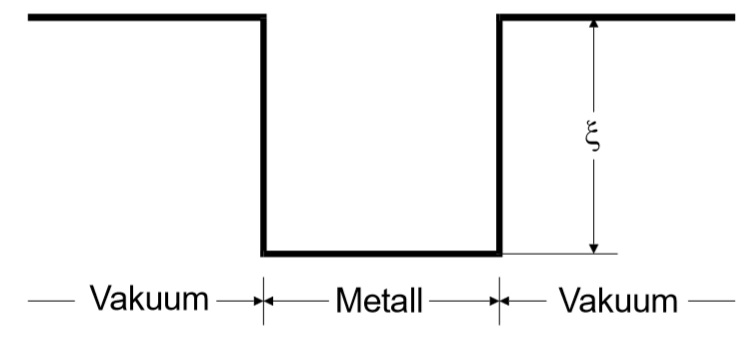
\includegraphics[height=4.0cm]{data/abb1.jpg}
    \caption{Potentialtopf-Modell eines Metalles. \cite{V504}}
    \label{fig:abb1}
\end{figure} \\
\noindent
Die Elektronen können nur diskrete, wenn auch sehr dicht beeinander liegende Energiewerte annehmen.
Als Teilchen mit halbzahligem Spin unterliegen die Elektronen eines Kristallgitters dem Pauli-Verbot, das besagt, dass jeder mögliche Zustand mit der Energie E von höchstens 2 Elektronen, die entgegengesetzten Spin haben müssen, eingenommen werden kann.
Das hat zur Konsequenz, dass selbst am absoluten Nullpunkt die Elektronen noch eine endliche Energie besitzen müssen, ganz im Gegensatz zur klassischen Statistik, die jedem Elektron im Mittel die Energie $\frac{3}{2}\text{k}T$ zuordnet.
Die Maximalenergie der Elektronen bei $T = 0$ ist abhängig von der Zahl n der Elektronen pro Volumeneinheit im Metall.
Man bezeichnet sie als Fermische Grenzenergie \xi.
Bei Zimmertemperatur ist für alle Metalle $\xi >> \text{k}T$.
Die Wahrscheinlichkeit dafür, dass im thermischen Gleichgewicht ein möglicher Zustand mit der Energie E besetzt ist, wird durch die Fermi-Diracsche Verteilungs-Funktion angegeben.
Sie hat die Gestalt
\begin{equation}
    \text{f}(\text{E}) = \frac{1}{\text{exp}\left(\frac{\text{E} - \xi}{\text{k}T}\right) + 1}
    \label{eqn:gl1}
\end{equation}
Ein Elektron muss mindestens die Energie $\xi + e_0 \Phi$ besitzen, um die Metalloberfläche zu verlassen, wie man im Verlauf der Gleichung \eqref{eqn:gl1} sieht in Abb. \ref{fig:abb2}.
Der Energiewert ist selbst beim Schmelzpunkt von Wolfram noch groß gegnüber $\text{k}T$, sodass die Exponentialfunktion aus Gleichung \eqref{eqn:gl1} die Zahl 1 weit übertrifft.
Für Elektronen mit höherer Energie als solche gilt in Näherung
\begin{equation}
    \text{f}(\text{E}) \approx \text{exp}\left(\frac{\xi - \text{E}}{\text{k}T}\right)
    \label{eqn:gl2}
\end{equation}
\begin{figure}
    \centering
    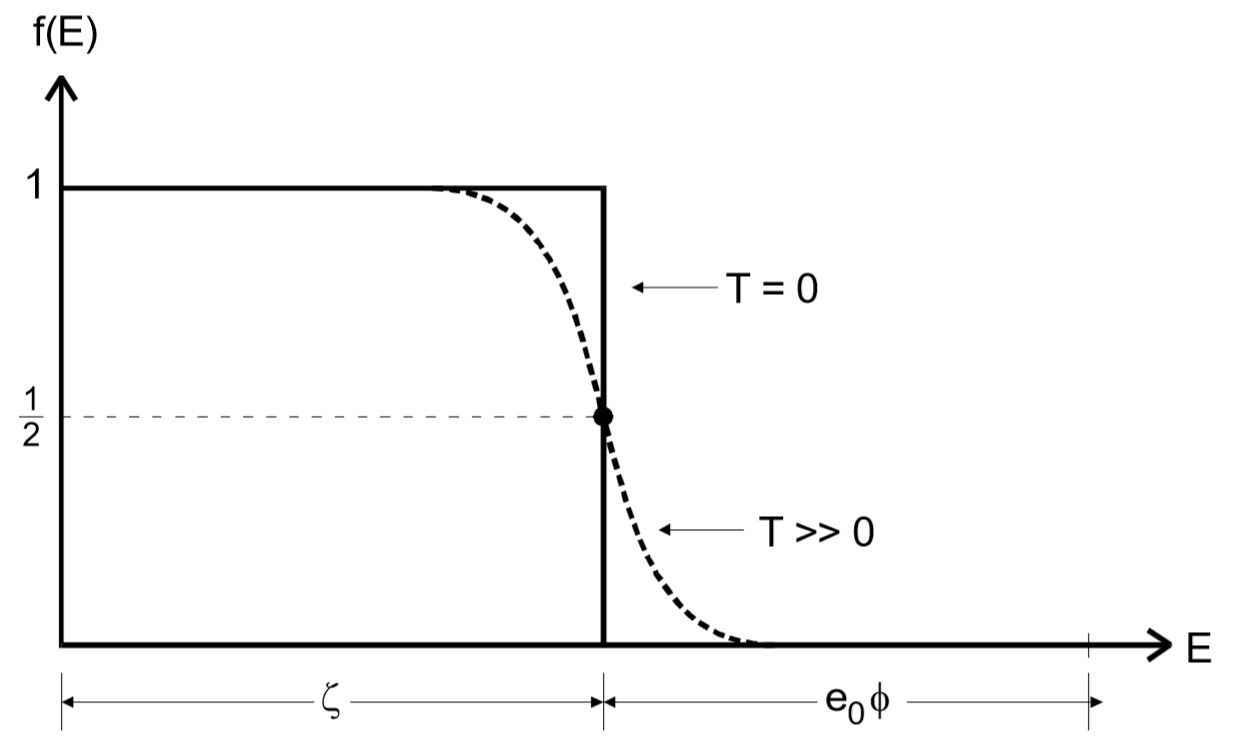
\includegraphics[height=4.0cm]{data/abb2.jpg}
    \caption{Verlauf der Fermi-Diracschen Verteilungsfunktion am absoluten Nullpunkt (durchgezogene Linie) und bei $T >> 0$ (gestrichelt). \cite{V504}}
    \label{fig:abb2}
\end{figure} \\
\noindent

\subsection{Sättigungsstromdichte}
Aus Gleichung \eqref{eqn:gl2} soll die Sättigungsstromdichte $j_s(T)$ in Abhängigkeit von der Temperatur errechnet werden.
Dazu wird ein Koordinatensystem mit Z-Achse senkrecht zur Oberfläche des Metalls eingeführt.
Durch die Zahl der Elektronen aus dem Volumenelement des Impulsraumes und einiger Beziehungen erhält man zuerst die Gleichung
\begin{equation}
    \text{d}\alpha = \frac{\partial \text{E}}{\partial p_z} \text{n}(\text{E}) \text{d}p_x \text{d}p_y \text{d}p_z = \text{n}(\text{E}) \text{d}\text{E} \text{d}p_x \text{d}p_y \text{d}p_z
    \label{eqn:gl3}
\end{equation}
Mit n(E) als Zahl der Elektronen pro Volumeneinheit und d\alpha als die Zahl der Elektronen aus dem Volumenelement des Impulsraumes.
Da jeder Quantenzustand im (sechsdimensionalen) Phasenraum das Volumen $\text{h}^3$ einnimmt, ergibt sich für n(E) der Ausdruck
\begin{equation}
    \text{n}(\text{E}) = \frac{2}{\text{h}^3}\text{f}(\text{E})
    \label{eqn:gl4}
\end{equation}
Somit können mit Gleichung \eqref{eqn:gl3} alle Elektronen die Metalloberfläche verlassen, deren deren Geschwindigkeitskomponente $v_z$ so groß ist, dass
\begin{equation}
    \frac{p_z^2}{2\text{m}_0} > \xi + e_0 \Phi
    \label{eqn:gl5}
\end{equation}
gilt.
Man erhält daher die gesuchte Stromdichte $j_s(T)$ aus Gleichung \eqref{eqn:gl3}, indem man alle Elektronen, deren Energiekomponente in Z-Richtung die Ungleichung \eqref{eqn:gl5} erfüllt, abzählt und den erhaltenen Zahlenwert mit der Elementarladung $e_0$ multipliziert.
Somit ist
\begin{equation}
    j_s(T) = 4 \pi \frac{e_0 \text{m}_0 \text{k}^2}{\text{h}^3}T^2 \text{exp}\left(\frac{-e_0 \Phi}{\text{k} T}\right)
    \label{eqn:gl6}
\end{equation}
Die Gleichung \eqref{eqn:gl6} wird als Richardson-Gleichung bezeichnet.

\subsection{Die Hohvakuum-Diode}
Die Messung des Sättigungsstromes einer emittierenden Metalloberfläche ist nur im Hochvakuum möglich, da sonst die freien Elektronen in Wechselwirkung mit den Gasmolekülen treten würden.
Sie besteht aus einem evakuierten Glaskörper, mit einer Glühkatode.
Durch einen Strom kann dieser auf eine Temperatur von 1000 bis 3000 K erhitzt werden.
Die aus der Drahtoberfläche austretenden Elektronen werden durch ein elektrisches Feld, das man zwischen der Kathode und einer ihr gegenüberstehenden zweiten Elektrode, der Anode, durch Anlegen einer äußeren Spannung erzeugt, abgesaugt.
\begin{figure}
    \centering
    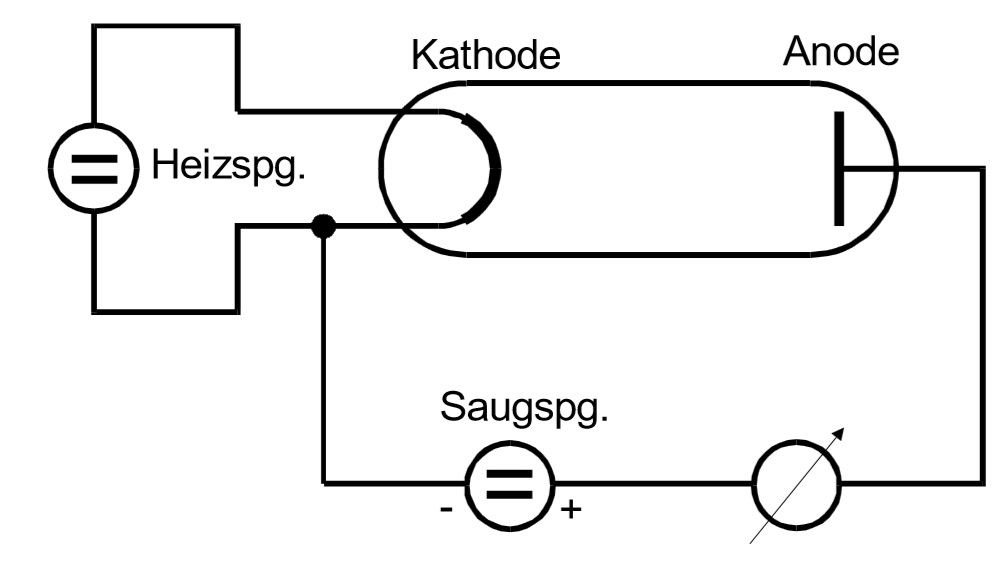
\includegraphics[height=4.0cm]{data/abb3.jpg}
    \caption{Beschaltung einer Hochvakuum-Diode. \cite{V504}}
    \label{fig:abb3}
\end{figure} \\
\noindent

\subsection{Die Langmuir-Schottkysche Raumladungsgleichung}
Der Anodenstroms hängt noch von der Anodenspannung ab, denn bei zu niedriger Spannung erreichen nicht alle emittierten Elektronen die Anode.
Erst bei hinreichend hoher Spannung wird ein von der Spannung unabhängiger Strom erreicht.
Durch die beschleunigte Bewegung der Elektronen auf die Anode zu gilt auch bei kleiner Spannung nicht das Ohmsche Gesetz.
Deswegen ist die Raumladungsdichte \rho der Elektronen eine Funktion des Ortes.
Diese wird zur Anode hin immer kleiner, aufgrund der Kontinuitätsbedingung, wobei j an jeder Stelle konstant ist.
\begin{equation}
    \text{j} = - \rho \text{v}
    \label{eqn:gl7}
\end{equation}
Die Raumladungsdichte \rho beeinflusst den Verlauf der Feldstärke zwischen Anode und Kathode, sie schirmt das Feld von der Kathode ab.
Der gemessene Diodenstrom ist somit kleiner als der nach Gleichung \eqref{eqn:gl6} zu erwartende Sättigungsstrom.
Für den quantitativen Zusammenhang wird von der Potentialgleichung ausgegangen:
\begin{equation}
    \Delta \text{V} = - \frac{1}{\epsilon_0} \rho
    \label{eqn:gl8}
\end{equation}
Zur Vereinfachung wird angenommen, dass Anode und Kathode unendlich ausgedehnt sind im Abstand a zueinander.
Durch Gleichung \eqref{eqn:gl7}, \eqref{eqn:gl8} und dem Energiesatz $\text{e}_0 \text{V} = m_0/2 \text{v}^2$ ergibt sich:
\begin{equation}
    \sqrt[4]{\text{V}^3(\text{x})} = \frac{3}{4} \sqrt{\frac{4 \text{j}}{\epsilon_0 \sqrt{2 \text{e}_0/\text{m}_0}}}\text{x}
    \label{eqn:gl9}
\end{equation}
Daraus folgt, dass das Potential nicht linear, sondern nach einem $\sqrt[3]{\text{x}^4}$-Gesetz ansteigt.
Deswegen verläuft die Feldstärke proportional zu $\text{x}^{\frac{1}{3}}$ und \rho proportional zu $\text{x}^{-\frac{2}{3}}$, zu sehen in Abb. \ref{fig:abb4}.
Gestrichelt eingezeichnet ist der raumladungsfreie Fall.
Aus Gleichung \ref{eqn:gl9} ergibt sich:
\begin{equation}
    \text{j} = \frac{4}{9} \epsilon_0 \sqrt{2 \text{e}_0/\text{m}_0} \frac{\text{V}^{3/2}}{a^2}
    \label{eqn:gl10}
\end{equation}
Anstelle des ohmschen Gesetzes ($j \propto V$) wächst hier j mit $\text{V}^{3/2}$.
Die Gleichung \eqref{eqn:gl10} wird als Langmuir-Schottkysche Raumladungsgesetz bezeichnet.
\begin{figure}
    \centering
    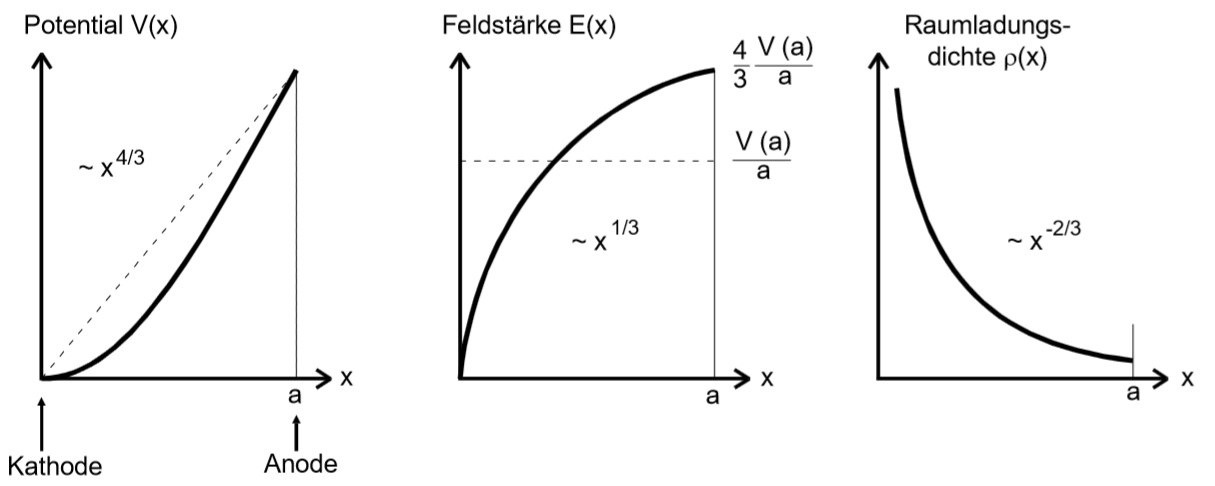
\includegraphics[height=5.0cm]{data/abb4.jpg}
    \caption{Ortsabhängigkeit des Potentials V, der Feldstärke E und der Raumladungsdichte \rho im Raumladungsgebiet einer Hochvakuumdiodenkennlinie. \cite{V504}}
    \label{fig:abb4}
\end{figure} \\
\noindent

\subsection{Anlaufstromgebiet einer Hochvakuumdiode}
Auch bei V=0 wird noch ein geringer Anodenstrom gemessen.
Dieser entsteht durch die Eigengeschwindigkeit der Elektronen, die sie beim Verlassen der Kathode besitzen.
Nach Gleichung \eqref{eqn:gl1} gibt es bei $T>0$ endlich viele Elektronen, deren Energie größer als die Austrittsarbeit ist.
Den Energieüberschuss
\begin{align*}
    \Delta \text{E} = \text{E} - \left(\xi + \text{e}_0 \Phi \right)
\end{align*}
findet man als kinetische Energie der emittierten Elektronen.
Diesen Strom wird als Anlaufstrom bezeichnet.
Es ist zu berücksichtigen, dass auch das Anodenmaterial eine Austrittsarbeit $\Phi_A$ besitzt.
Durch die elektrisch leitende Verbindung zwischen Anode und Kathode außerhalb der Diode werden die Fermi-Oberflächen (d.h. die Stelle E = \xi auf der Energieachse) der Metalle auf die gleiche Höhe gebracht.
Mit einem äußeren Potential V verschieben sich $\text{e}_0 \text{V}$ gegeneinander.
\begin{figure}
    \centering
    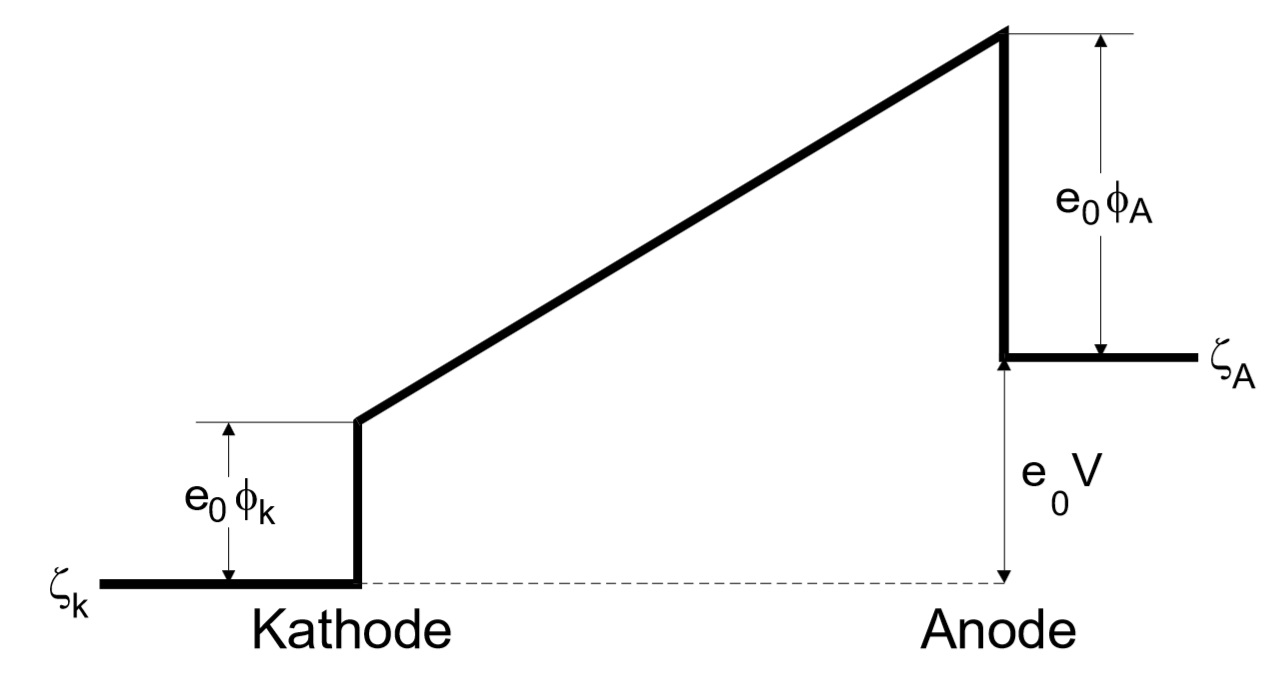
\includegraphics[height=5.0cm]{data/abb5.jpg}
    \caption{Potentialverhältnisse in einer Hochvakuumdiode im Bereich ihres Anlaufstromgebietes  \cite{V504}}
    \label{fig:abb5}
\end{figure} \\
\noindent
Da die Zahl der Leitungselektronen, deren Energie zwischen E und E+dE liegt, nach Gleichung \ref{eqn:gl2} angenähert exponentiell von E abhängt, besteht auch eine entsprechende Abhängigkeit der Anlaufstromstärke vom äußeren Potential V:
\begin{align*}
    \text{j}(\text{V}) = \text{j}_0 \text{exp} \left(\frac{\text{e}_0 \Phi_A + \text{e}_0 \text{V}}{y}\right)
\end{align*}

\subsection{Kennlinie der Hochvakuumdiode}
Nach den vorherigen Ausführungen lässt sich die Kennlinie in drei Abschnitte unterteilen.
Anlauf-, Raumladungs- und Sättigungsstromgebiet.
Das erstere ist durch einen exponentiellen Zusammenhang zwischen I und V gekennzeichnet.
Daran schließt sich das Raumladungsgebiet an, in dem eine $\sqrt{\text{V}^3}$-Abhängigkeit zu beobachten ist.
Dieses Gebiet wird durch das Sättigungsstromgebiet abgelöst, weil die Raumladungsgleichung nicht für beliebig hohe Anodenspannungen gilt.
\begin{figure}
    \centering
    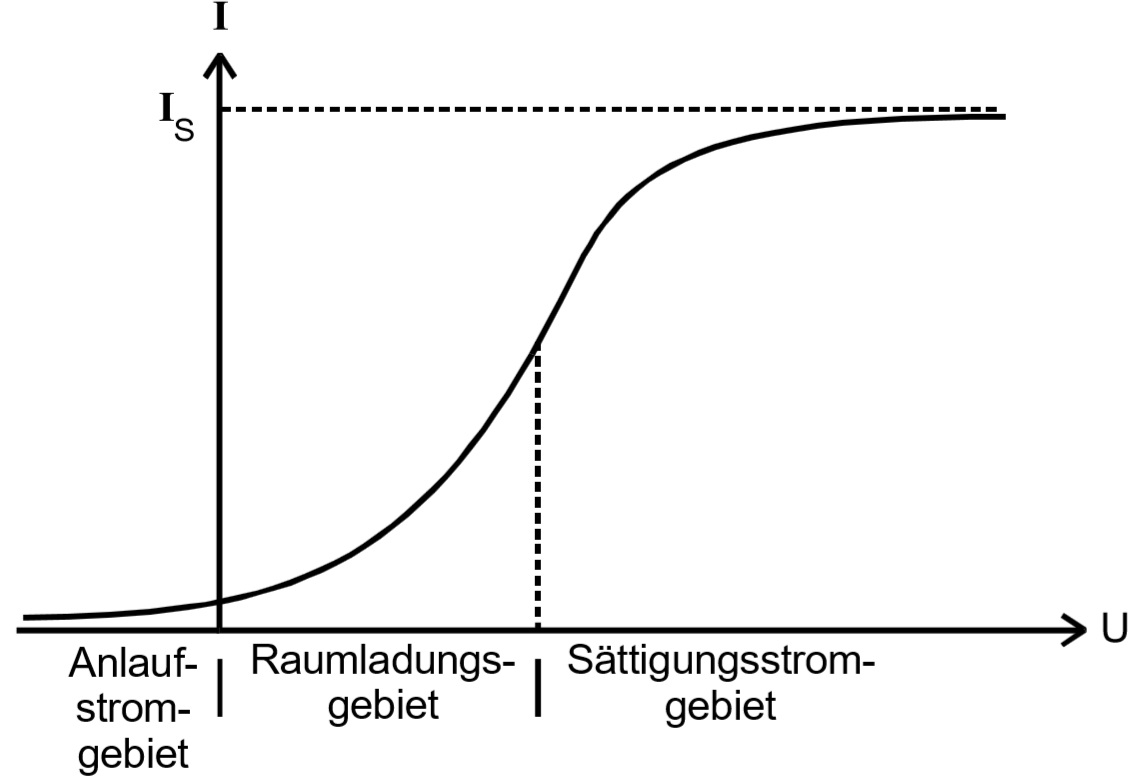
\includegraphics[height=5.0cm]{data/abb6.jpg}
    \caption{Kennlinie einer Hochvakuumdiode \cite{V504}}
    \label{fig:abb6}
\end{figure} \\
\noindent

\section{Aufbau}
\begin{figure}
    \centering
    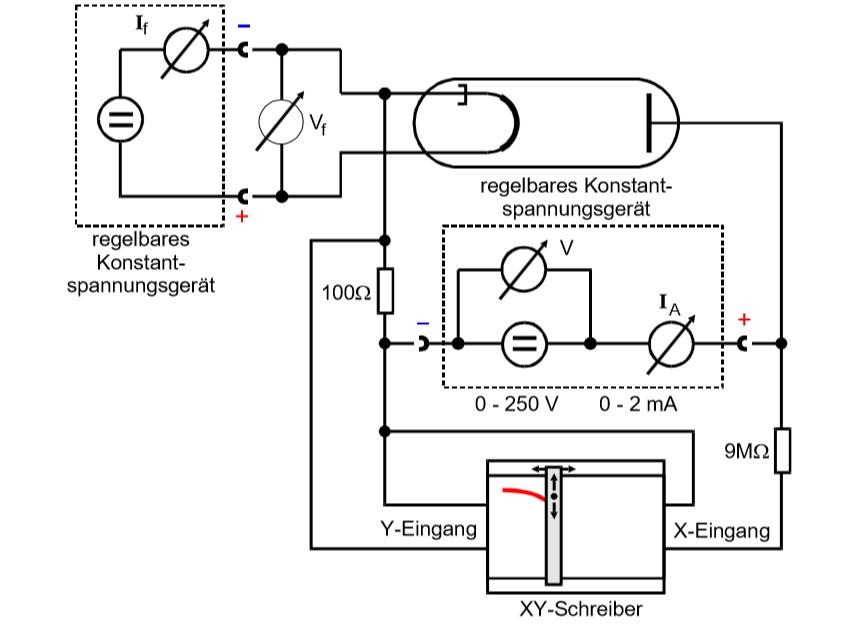
\includegraphics[height=5.0cm]{data/abb7.jpg}
    \caption{Schaltung zur Aufnahme von Diodenkennlinien \cite{V504}}
    \label{fig:abb7}
\end{figure}
Das Schaltbild für diesen Versuch ist in Abbildung \ref{fig:abb7} zu sehen.
Der in dieser Abbildung dargestellte XY-Schreiber wird nicht verwendet.
Von einem Konstantspannungsgerätes wird ein Heizstrom $I_\text{f}$ von ca. 2-3 A erzeugt.
Über ein seperates Voltmeter wird die Heizspannung $V_\text{f}$ abgelesen.
Die Anodenspannung $V_\text{A}$ und die Anodenstromstärke $I_\text{A}$ werden einem weiteren regelbaren Konstantspannungsgerät entnommen, in das entsprechende Messgeräte eingebaut sind.
